\documentclass{jhwhw}
\author{Ian Malerich}
\title{Math 481: Homework 2}

\usepackage{amssymb, amsfonts, mathtools, graphicx, breqn, minted}
\usemintedstyle{friendly}
\graphicspath{ {png/} }

\begin{document}
\raggedright

\problem{}

    Find the characteristic equation and reduced characteristic equation of the 3-step method
    $$
	y_{n+1} = -\frac{27}{11}y_n + \frac{27}{11}y_{n-1} + y_{n-2} + 
	h\biggr[\frac{3}{11}f_{n+1} + \frac{27}{11}f_n + \frac{27}{11}f_{n-1} + \frac{2}{11}f_{n-2}\biggr]
    $$

    Find the (exact) roots of the reduced characteristic equation, and determine if this method
    is stable for small $h\lambda$ or not.

\solution
    
    First let us rewrite the method as
    $$
	y_{n+1} + \frac{27}{11}y_n - \frac{27}{11}y_{n-1} - y_{n-2} =
	h\biggr[\frac{3}{11}f_{n+1} + \frac{27}{11}f_n + \frac{27}{11}f_{n-1} + \frac{2}{11}f_{n-2}\biggr]
    $$

    Note that for this method we have 
    $$
	a_0 = -1, a_1 = -\frac{27}{11}, a_2 = \frac{27}{11}
    $$

    Which produces the characteristic polynomial
    \begin{align*}
	p(z) &= z^3 + \frac{27}{11}z^2 - \frac{27}{11} - 1 \\
	&= \frac{1}{11}(z-1)(11z^2 + 38z+11) \\
	&= \frac{1}{11}(z-1)
	    (z + \frac{1}{11}(19 + 4\sqrt{15}))
	    (z - \frac{1}{11}(4\sqrt{15} - 19))
    \end{align*}

    From this we find the zeros for the characteristic polynomial
    $$
	z = 1,
	z = -\frac{1}{11}(19 + 4\sqrt{15}),
	z = \frac{1}{11}(4\sqrt{15} - 19)
    $$

\problem{}

    The IVP
    \begin{align*}
	y' &= -y + 2e^{-t}\cos(2t) \\
	y(0) &= 0
    \end{align*}
    has the true solution $y(t) = e^{-t}\sin(2t)$. \\
    Solve it numerically from t=0 to t=5, using
    \begin{enumerate}
	\item the classical 4-stage Runge-Kutta method with h=0.2
	\item a PECE predictor-corrector method based on 4-step AB, 3-step AM, h=0.2 \\
	    Use RK values from part (a) for the startup.
	\item the Matlab built-in ODE45. This routine will pick its own steps.
    \end{enumerate}

\solution
    \begin{center}
	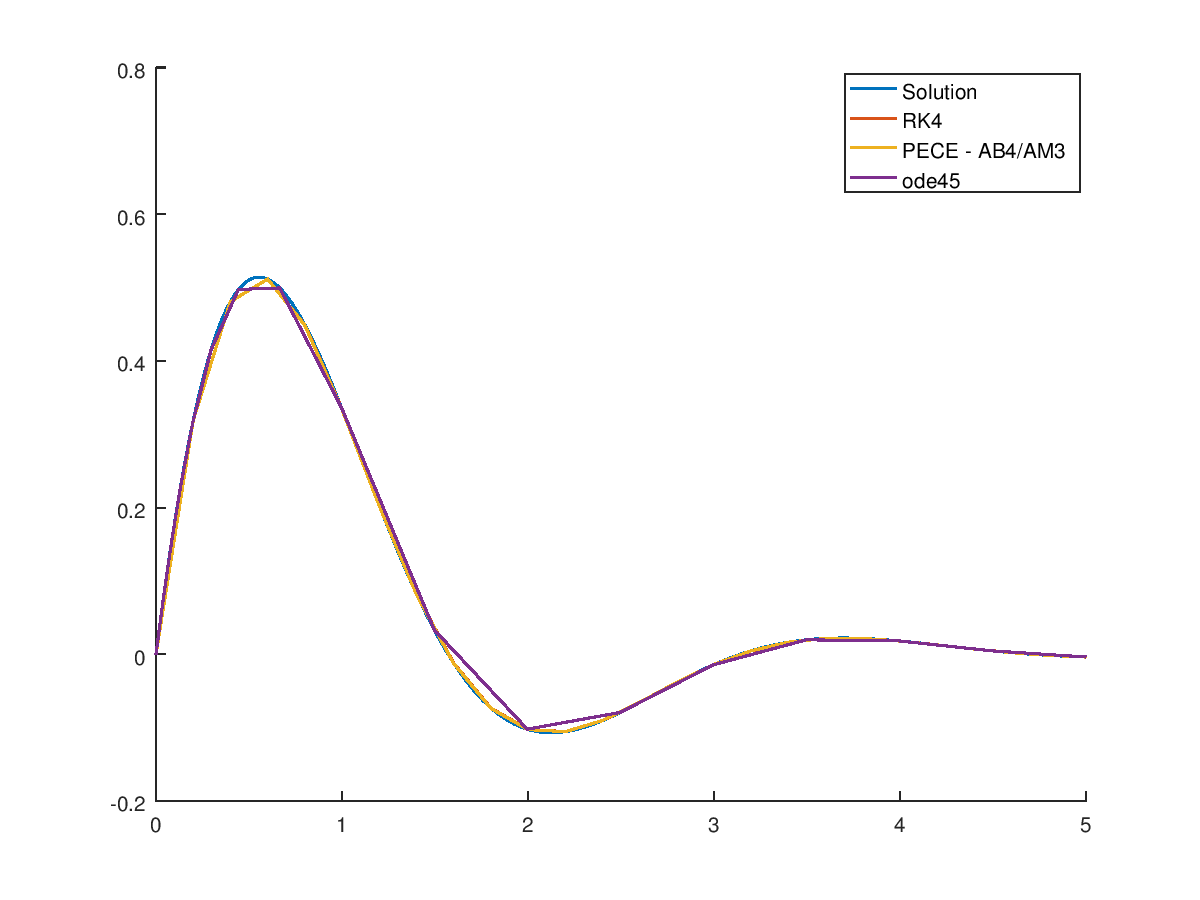
\includegraphics[scale=0.95]{p1_0_2}

	\begin{tabular}[pos]{|l|r|r|r|r|}
	    \hline
	    & Actual	& RK4			& PECE - AB4/AM3	& ODE45 (h unknown) \\ \hline
	    h = 0.2 &&&& \\ \hline
	    Value	& -0.013911	& -0.013911		& -0.013776  & -0.014068 \\ \hline
	    Error	& 		& $2.1822*10^{-7}$	& $1.3560*10^{-4}$ & $1.5663*10^{-4}$\\ \hline
	    h = 0.1 &&&& \\ \hline
	    Value	& -0.013911	& -0.013911		& -0.013908 & \\ \hline
	    Error	& 		& $1.2907*10^{-8}$	& $3.3871*10^{-6}$ & \\ \hline
	\end{tabular}
    \end{center}

    \inputminted[linenos,frame=lines,framesep=2mm]{octave}{p2.m}

\problem{}

    Use the Matlab routine $fzero$ or something comparable to find the two solutions of
    $$ e^x - x - 2 = 0.$$
    There is one positive and one negative solution.

\solution
    
    TODO

\end{document}
